% -*- TeX-engine: default; -*-
\documentclass[10pt,sigconf]{acmart}
\usepackage[font=footnotesize]{subcaption}
\usepackage[utf8]{inputenc}
\usepackage[T1]{fontenc}
\usepackage{url}
\usepackage{booktabs}
\usepackage{xcolor}
\usepackage{enumitem}
\usepackage{algorithm}
\usepackage[noend]{algpseudocode}

\setcopyright{rightsretained}
\acmYear{2018}
\copyrightyear{2018}
\acmConference[CoNEXT'18]{ACM CoNEXT 2018}{December 2018}{Heraklion/Crete, Greece}

\begin{document}
\title{The eXpress Data Path: Programmable Packet Processing for the Linux Kernel}
%\author{Toke Høiland-Jørgensen}
%\affiliation{%
%  \institution{Karlstad University}}
%\email{toke.hoiland-jorgensen@kau.se}
%
%\author{Jesper Dangaard Brouer}
%\affiliation{%
%  \institution{Red Hat}}
%\email{brouer@redhat.com}
%
%\author{Daniel Borkmann}
%\affiliation{%
%  \institution{Cilium.io}}
%\email{daniel@cilium.io}
%
%\author{John Fastabend}
%\affiliation{%
%  \institution{Cilium.io}}
%\email{john@cilium.io}
%
%\author{Tom Herbert}
%\affiliation{%
%  \institution{Quantonium Inc.}}
%\email{tom@herbertland.com}
%
%\author{David Ahern}
%\affiliation{%
%  \institution{Cumulus Networks}}
%\email{dsahern@gmail.com}
%
%\author{David Miller}
%\affiliation{%
%  \institution{Red Hat}}
%\email{davem@redhat.com}
%
%\renewcommand{\shortauthors}{T. Høiland-Jørgensen et al.}
\author{A. Anonymous}
\affiliation{%
       \institution{Institution}
       \country{Country}}
\email{anon@example.org}

\renewcommand{\shorttitle}{The eXpress Data Path}
\captionsetup{font+=small}

\begin{abstract}
  % Max abstract length is 200 words
  Programmable packet processing is most often implemented using kernel bypass
  techniques, where a userspace application takes complete control of the
  networking hardware to avoid expensive context switches between kernel and
  userspace. However, in this model the processing application has to either
  perform cumbersome re-injection of packets into the kernel, or handle all
  network traffic itself, making high-speed packet processing an all-or-nothing
  proposition.

  To overcome this limitation, we propose a novel approach to programmable
  packet processing where the kernel itself provides a safe execution
  environment for custom packet processing applications, executed in device
  driver context. This system, called the eXpress Data Path (XDP), has recently
  been merged into the mainline Linux kernel and provides a fully integrated
  solution working in concert with the kernel's network stack. In XDP,
  applications written in higher level languages such as C are compiled into
  custom bytecode which the Linux kernel statically analyses for safety, and
  translates into native instructions.

  We show that XDP achieves single-core packet processing performance as high as
  25 million packets per second, and illustrate the flexibility of the
  programming model through three example use cases: inline DDoS protection,
  layer-3 routing and layer-4 load balancing.
\end{abstract}

% TODO: Add ccsxml tags and update keywords

\keywords{XDP, BPF, Programmable Networking}
\maketitle

\section{Introduction}%
\label{sec:introduction}
High-performance packet processing in software has very tight bounds on the time
spent processing each packet ($\simeq6$~ns per packet at 100 Gbps). Network
stacks in general purpose operating systems typically perform too many
operations per packet to be able to keep up with this packet rate, which has led
to increased popularity of special-purpose toolkits for software packet
processing, such as the Data Plane Development Kit (DPDK)~\cite{dpdk}. Such
toolkits generally bypass the operating system completely, instead passing
control of the network hardware directly to the network application and
dedicating one, or several, CPU cores exclusively to packet processing.

The kernel bypass approach can significantly improve performance, but has the
drawback that it is more difficult to integrate with the existing networking
stack, and applications have to re-implement a great deal of functionality
otherwise provided by the operating system kernel. In the worst case, this leads
to the need to operate two separate stacks; one to perform high-speed packet
processing and one to run normal application or container workloads, leading to
increased systems complexity, management and maintainability costs, and at the
same time blur strict security boundaries otherwise provided by the operating
system kernel. The latter is in particular problematic as today's infrastructure
is moving towards container-based workloads coupled with orchestration systems
such as Docker or Kubernetes, where the kernel plays a dominant role in resource
abstraction and isolation.

As an alternative to the all-or-nothing kernel bypass packet processing
technique, we present a system that adds programmability directly in the
operating system networking stack in a cooperative way, making it possible to
perform high-speed packet processing that integrates seamlessly with existing
systems, while selectively leveraging functionality in the operating system.
This framework, called the eXpress Data Path (XDP), works by defining a limited
execution environment in the form of a virtual machine running a custom bytecode
that is based on an extended version of the Berkeley Packet Filter. This allows
programs to run directly in the device driver context, before the kernel
performs any other packet processing tasks. The kernel ensures safety and
performance by statically verifying the program before it is loaded, and
dynamically Just-in-Time-compiling the virtual machine bytecode in to native
machine instructions.

XDP has been gradually integrated into the Linux kernel over the last several
releases. However, no complete architectural description of the system as a
whole exists in the literature. In this work we present such a high-level design
decription of XDP, its capabilities and how it integrates with the rest of the
Linux kernel. Our performance analysis shows raw packet processing performance
on a single core of up to 25 million packets per second. In addition,
performance scales both downwards, by decreasing CPU usage as the traffic load
drops, and upwards, by increasing performance with the number of cores dedicated
to packet processing.

Because of its integration with the kernel's networking stack, and its high
performance, XDP allows for implementing applications such as DDoS protection
and load balancing that previously required their own networking appliance to
run directly on application servers. It also enables a hybrid approach, where
certain fast path processing is offloaded to XDP while retaining normal network
stack processing for other packets. In addition, XDP supports atomic application
updates without traffic interruption or service restarts, which allows for high
performance processing without sacrificing flexibility.

To illustrate the various facets of XDP, we supplement our synthetic performance
benchmarks with three non-exhaustive examples of real-world use cases that can
be implemented in XDP: inline DDoS protection on a hypervisor host or
application server; full layer-3 packet forwarding capabilities; and layer-4
load balancing by encapsulating packets and reinjecting them into the network.

The rest of this paper is structured as follows: Section~\ref{sec:related-work}
first outlines related work. Section~\ref{sec:design} then presents the design
of XDP and Section~\ref{sec:perf-eval} presents the raw packet processing
performance analysis. Section~\ref{sec:usecases} presents the real-world use
cases and their performance. Finally, Section~\ref{sec:limitations} presents
current limitations of XDP and future work, and Section~\ref{sec:conclusion}
concludes.

\section{Related Work}%
\label{sec:related-work}

Programmable packet processing continues to gain momentum as the performance
attainable on commodity hardware rises, and costs fall. Programmable hardware
devices such as the NetFPGA~\cite{lockwood2007netfpga}, allows this processing
to continue to happen on specialised hardware, by exposing an API that makes it
possible to run arbitrary packet processing tasks on the FPGA-based dedicated
hardware. The P4 language~\cite{bosshart2014p4} seeks to extend this
programmability to a wider variety of packet processing hardware.

However, even though specialised hardware has begun to gain data plane
programmability, the flexibility of commodity hardware has obvious advantages,
and as performance increases and cost decreases, this becomes ever more popular.
To achieve the maximum possible performance in this setting, it is necessary to
remove any bottlenecks between the networking interface card (NIC) and the
program performing the packet processing. Since one of the main sources of
performance bottlenecks is the interface between the operating system kernel and
the userspace applications running on top of it (because of the high overhead of
a system call), most packet processing frameworks are focused on managing this
in various ways. The approaches taken fall into three broad categories: (a)
implementing parts of the application as a module inside the kernel itself, (b)
providing an interface for userspace to access packet data with lower overhead
than with traditional sockets, or (c) bypassing the kernel entirely and handing
over control of the networking device directly to userspace.

In the first category, systems such as the OpenVswitch~\cite{openvswitch}
virtual switch and the Click~\cite{martins2014clickos} software router provide
kernel modules that offload part of their functionality into the kernel. These
are implemented as loadable kernel modules that provide configuration APIs to
userspace, but performs packet processing directly in the kernel. The drawback
of implementing packet processing applications in this way, is that it requires
deep familiarity with internal kernel APIs, and a failure of the network
processing application in most cases leads to a failure of the entire system.
Both OpenVswitch and Click are general frameworks that can be configured to do a
variety of tasks, which makes this cost easier to bear; thus it is no
coincidence that these are the prominent examples of the in-kernel processing
approach.

In the second category, various systems introduce kernel modules that do not
perform packet processing themselves, but instead focus on moving packet data
out to userspace with as little overhead as possible, typically via shared
memory. This allows the packet processing application to operate in userspace
with no risk of crashing the system. Examples of this approach include
PF\_RING~\cite{deri2009modern}, the Packet I/O engine that is part of
PacketShader~\cite{han2010packetshader}, and the Netmap~\cite{rizzo2012netmap}
framework. The drawback of this approach is that even if the frameworks
mentioned above improve performance significantly, they still lack behind in
performance compared to kernel bypass
solutions~\cite{gallenmuller_comparison_2015}.

In the third category of kernel bypass techniques, we find the PF\_RING ZC
module~\cite{pfringzc}, the hardware-specific Solarflare
OpenOnload~\cite{openonload} and, most prominently, the DataPlane Development
Kit (DPDK)~\cite{dpdk}, which started out as an Intel-specific hardware support
package, but has since seen a wide uptake under the stewardship of the Linux
Foundation. This approach offers excellent performance, but has the drawback
that it is more difficult to integrate with the rest of the system, as mentioned
in the introduction.

XDP takes the first approach to lowering overhead, and places the packet
processing in kernel device driver context, before any other processing. This
means that not only the overhead of passing every packet to userspace is
avoided, but also the overhead of the regular kernel networking stack. By using
a custom byte code format for the programming, which can be statically verified
to not adversely affect the functioning of the rest of the kernel, most of the
fragility issues normally faced by in-kernel packet processing implementations
(mentioned above) are avoided. In addition, the byte code format and execution
context are part of the kernel Application Binary Interface (ABI) to userspace,
which means that the usual stability guarantees of kernel ABI applies; and so
application do not have to keep up with future changes in the kernel to be able
to continue to function.

While XDP is primarily an instance of the first of the three approaches metioned
above, it also borrows aspects from the other two: For applications that prefer
receiving the full packet contents in userspace, XDP also contains features that
offer higher performance when redirecting packets to applications, virtual
machines and containers running in userspace. This include the ability to bypass
parts of the network stack processing, and even to perform zero-copy transfer of
packets to userspace applications using a special socket type. These facilities
roughly correspond to the second approach mentioned above. Finally, XDP applies
some of the same performance enhancing techniques used by the kernel bypass
frameworks, such as packet batching and the ability to process packets
immediately after they are received from the hardware.

%FIXME: Cite the "lessons learned with BPF" paper.

\section{The design of XDP}
\label{sec:design}
XDP is designed to integrate with the Linux networking stack, enhancing it with
high-performance programmable hooks in strategic places. This makes it possible
to take advantage of the extensive and robust features of the operating system,
while adding custom packet processing as required. For this reason, XDP should
not be seen as a monolithic system one injects a single program into, but rather
a composition of individual parts that operate in concert to achieve the desired
outcome.

\begin{figure}[t]
\centering
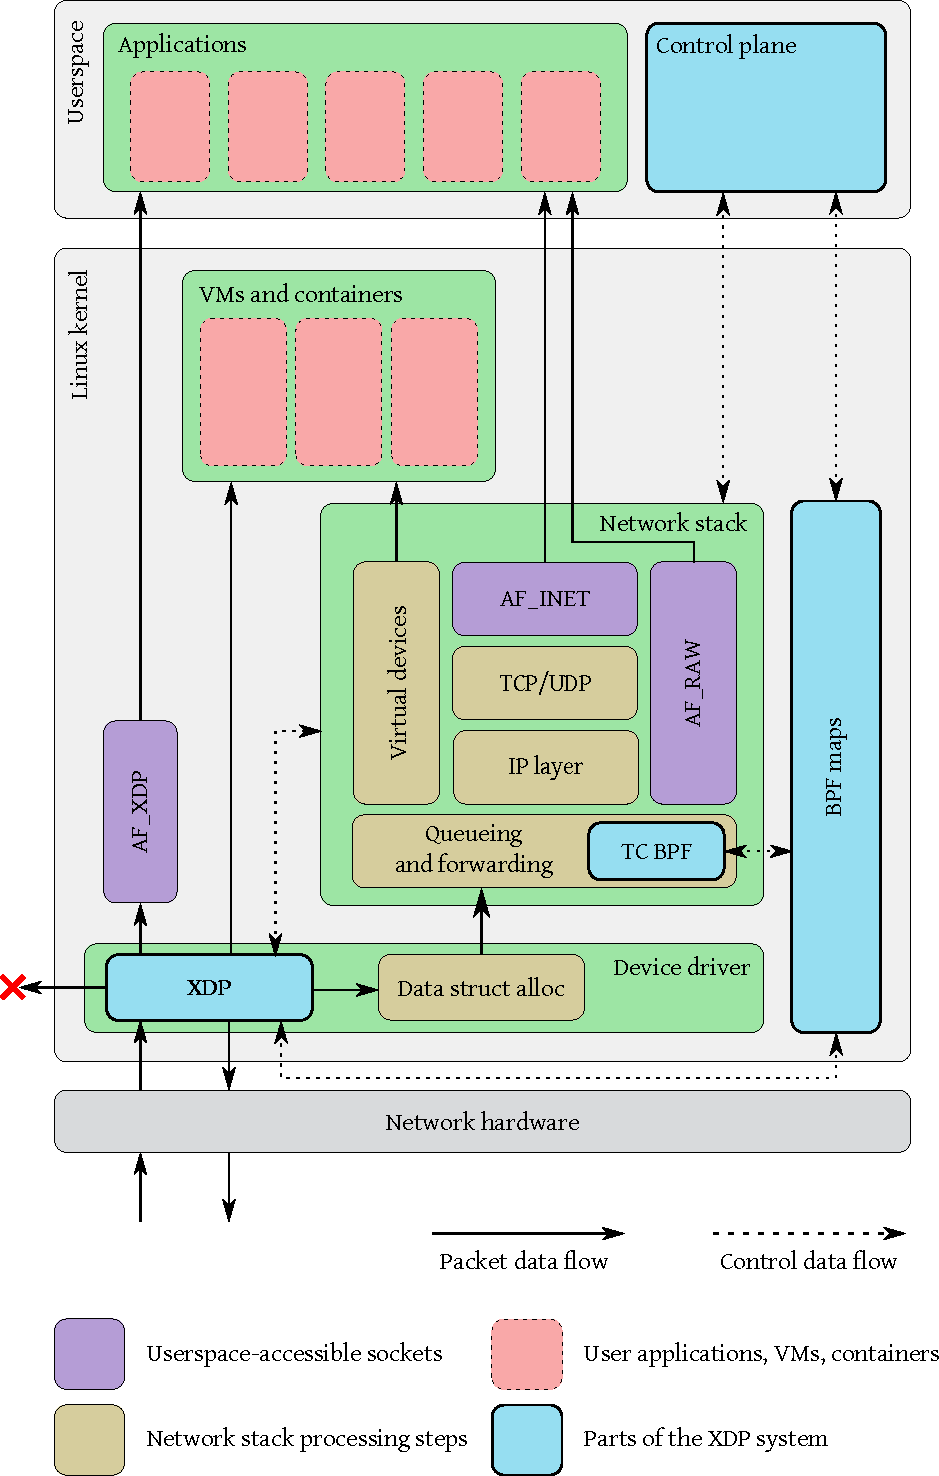
\includegraphics[width=\linewidth]{figures/kernel-diagram.pdf}
\caption{\label{fig:xdp-kernel} Diagram of how XDP integrates into the Linux
  kernel network receive path.}
\end{figure}


This section describes the various parts of the XDP system and how they fit
together. We begin with a high-level overview of the XDP programming model and
how various features of the kernel combine to form a powerful programmable data
plane. Following this, we look in detail at the extended BSD Packer Filter
(eBPF) virtual machine providing the execution model, and the in-kernel verifier
that ensures the safety of loaded eBPF programs. Finally, we give an overview of
some of the performance optimisations that are part of the XDP system, and which
help ensure high performance.

Figure~\ref{fig:xdp-kernel} shows a diagram of how XDP integrates into the Linux
kernel, and Figure~\ref{fig:xdp-execution} shows the execution flow of a typical
XDP program. Together, they give an overview of the full XDP system, and they
will be referenced throughout the exposition below.

\subsection{The XDP programming model}
\label{sec:prog-model}
The XDP system enables high-performance packet processing integrated tightly
with the rest of the Linux networking stack. This makes XDP unique compared to
other high-performance software packet processing frameworks, because it makes
it possible to selectively leverage features already implemented in Linux, while
writing custom programs to perform application-dependent processing, or to
accelerate certain parts of the data path. This section gives a conceptual
overview of the XDP programming model, explaining how the different parts fit
together.

\begin{figure*}[t]
\centering
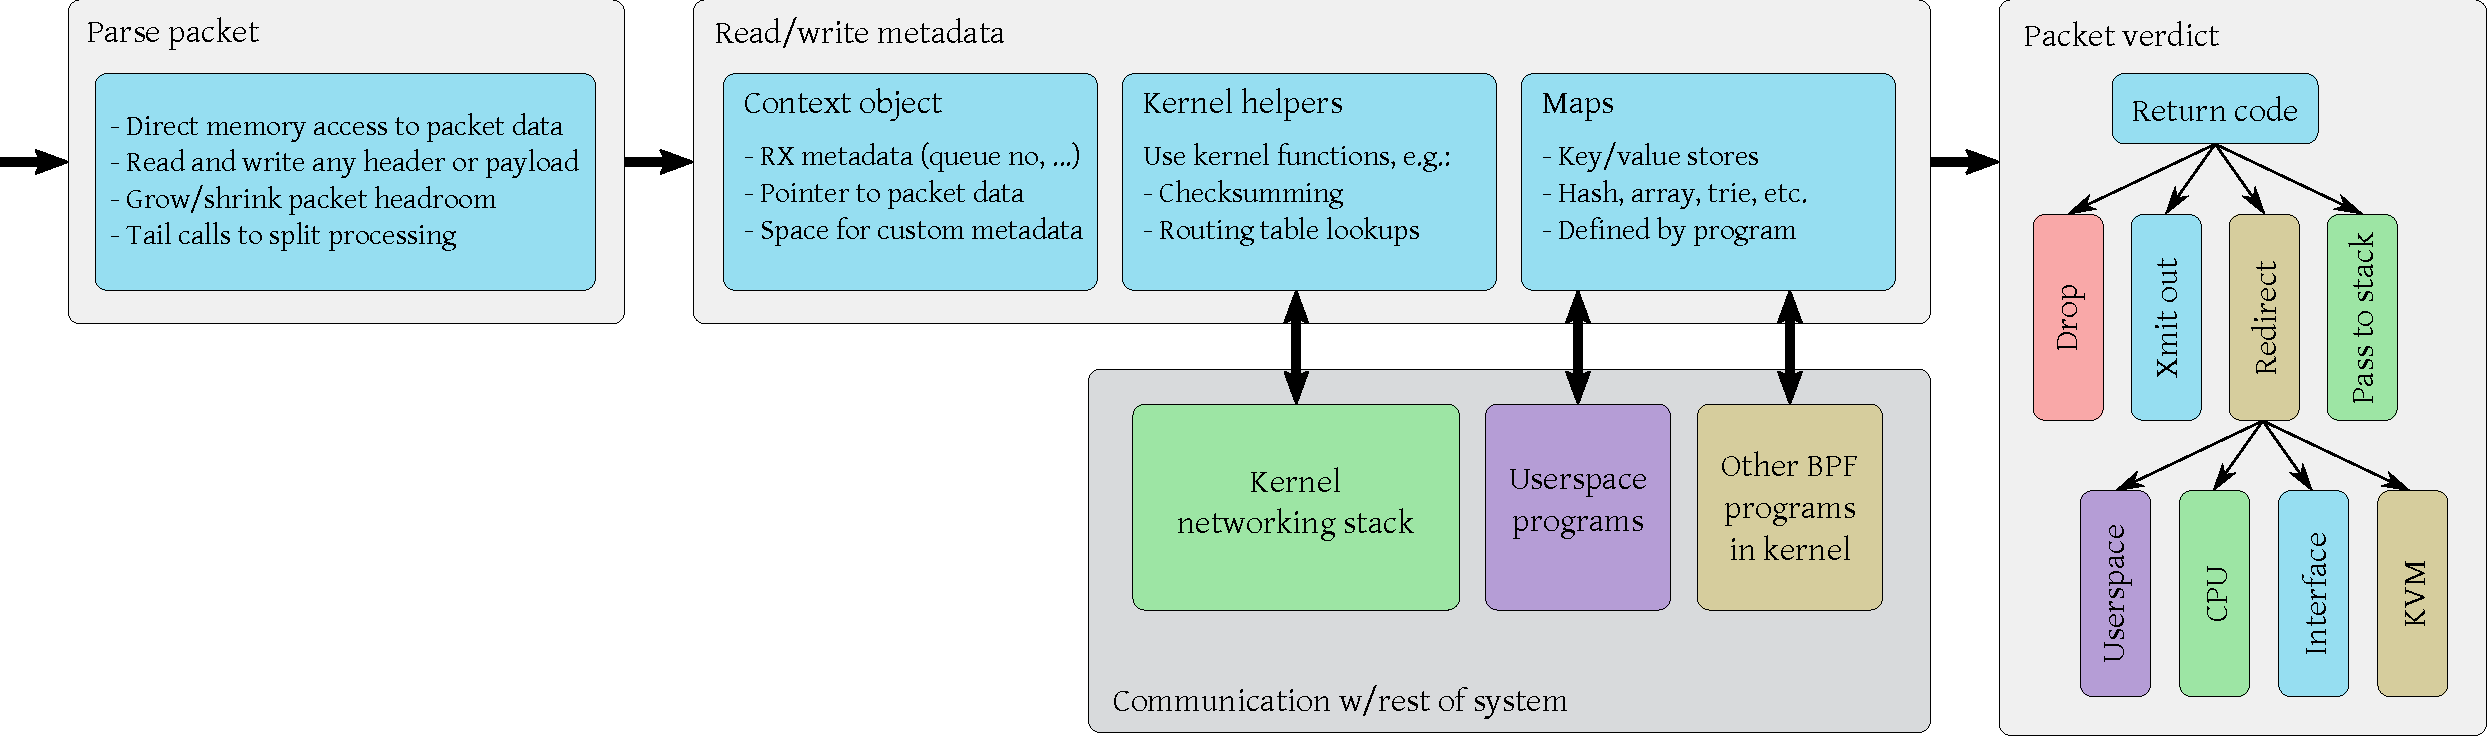
\includegraphics[width=\linewidth]{figures/xdp-execution-diagram.pdf}
\caption{\label{fig:xdp-execution} Execution diagram of a typical XDP program.
  When a packet arrives, the program starts by parsing packet headers to extract
  the information it will react on. Based on this, combined with information
  from one or more of the metadata facilities, a packet can be rewritten and a
  final verdict for the packet determined. The program can alternate between
  packet parsing, metadata lookup and rewriting, all of which are optional. The
  final verdict is given in the form of a program return code.}
\end{figure*}


An XDP program is run in the eBPF virtual machine and is entirely event driven.
The program is executed directly in context of the device driver, without
context switching to userspace. As shown in Figure~\ref{fig:xdp-kernel}, the
program is executed at the earliest possible moment after a packet is received
from the hardware, before the kernel allocates its per-packet \emph{sk\_buff}
data structure or performs any parsing of the packet. This allows for high
performance, but the program has to parse raw packet data itself.

Figure~\ref{fig:xdp-execution} shows the various processing steps an XDP program
can perform. The program starts its execution with access to a pointer to a
context object. This object contains pointers to the raw packet data (direct
packet access bounds are checked by the verifier), along with metadata fields
describing which interface and receive queue the packet came in on, etc.
%
The program typically begins by parsing packet data, can invoke
BPF helper functions (e.g., to perform a map lookup), or can pass control to a
different XDP program, through tail calls, thus splitting processing into
logical sub-units (based on, say, IP header version). The context object also
contains a pointer to a special memory area is available for XDP to store
arbitrary metadata that will be available to other XDP programs, as well as to
other parts of the kernel and userspace (under certain circumstances). The
program can also write any parts of the packet data buffer, including expanding
or shrinking the packet to add or remove headers.
%
% FIXME: More clear desc of header vs tail expand vs shrink support
%
% ALSO Describe: that we recently added truncating the packet tail
% length, but not expanding the tail.
%
These three steps (reading,
metadata processing, and writing packet data) correspond to the light grey boxes
on the left side of Figure~\ref{fig:xdp-execution}, and can of course alternate
and repeat in a arbitrary ways.

Similar to a regular userspace program, an XDP program ends its execution with a
return code, instructing the kernel what to do with the packet. This is shown on
the right-hand side of the figure. There are three simple return codes which
either drop the packet (\texttt{XDP\_DROP}), immediately re-transmit it out the
same network interface (\texttt{XDP\_TX}), or allow the packet to be processed
by the kernel networking stack (\texttt{XDP\_PASS}).  In addition to these
simple actions, the XDP program can \emph{redirect} the packet
(\texttt{XDP\_REDIRECT}), which controls its further processing (covered in
Section~\ref{sec:redir}).

During its execution, an XDP program also has access to kernel facilities that
provide helper functions and additional metadata. These allow the XDP program to
gather additional metadata through helper functions and maps (dotted lines in
Figure~\ref{fig:xdp-kernel} and the top part of Figure~\ref{fig:xdp-execution}).
%
% I'm not sure it's 100% correct to call helper functions "callbacks"?
%
% Please correct me: AFAIK the verifier translates helper ID numbers into
% real kernel function calls (change insn->imm = bpf_func_proto->func).
% (After the verifier have checked that R1-R5 argument passing registers
% are correct and compliant).
% (based on reading kernel/bpf/verifier.c function call fixup_bpf_calls
%
% I'm not sure if the CPU still sees this as an indirect-function pointer call,
% when JIT translated?
%
Helper functions are callbacks implemented in the kernel that an XDP program can
call to make use of kernel functionality in its processing. These helpers
serve various purposes, ranging from simple checksum computation and hashing, to
full access to the kernel routing table. New helpers are actively been added by
the kernel development community in response to user requests, continuously
expanding the functionality that XDP programs can make use of.

Maps are key/value stores that are defined by the user before loading an XDP
program, and can be referred to from within the eBPF code. Maps are shared, both
between different eBPF programs running at various places in the kernel, as well
as between eBPF and userspace. The map types include generic hash maps, arrays
and radix trees, as well as specialised types containing pointers to eBPF
programs (used for tail calls), or even recursive pointers to other maps. Maps
serve several purposes: they are a persistent data store between invocations of
the same eBPF program; a global coordination tool, where eBPF programs in one
part of the kernel can update state that changes the behaviour in another; and a
communication mechanism between userspace programs and the kernel eBPF programs,
similar to the communication between control plane and data plane in other
programmable package processing frameworks.

Another piece of the XDP picture is the ability to run eBPF programs in other
parts of the kernel. These include packet processing in the Traffic Control (TC)
subsystem, where eBPF programs can filter packets after they have been parsed by
the kernel, or before they are passed to the hardware from applications. This is
marked as ``TC BPF'' in Figure~\ref{fig:xdp-kernel}. In addition, eBPF programs
can be attached to various places in the kernel that are unrelated to networking
(not shown in the figures). These include \emph{cgroups}, which control resource
usage for groups of processes (used for implementing containers on Linux, for
instance), as well the \emph{tracepoint} and \emph{kprobe} introspection
subsystems which allow attaching eBPF programs to arbitrary kernel functions.
Because all eBPF programs can share the same set of maps, this makes it possible
for XDP programs to react to arbitrary events in the kernel, for instance by
dropping packets if processing load increases. Because of this integration, the
XDP programming model is considerably more powerful than just the XDP programs
itself.

A final important feature of the XDP system is the ability to dynamically load
eBPF programs. Because the kernel manages the life cycle of all eBPF programs,
they can be dynamically loaded and reloaded at runtime. Combined with dynamic
dispatch to other programs using tail calls, this makes it possible to limit the
amount of processing actually performed on packets. A processing pipeline can
simply split its processing into separate XDP programs and dynamically load and
unload them as features are enabled or disabled through control plane
configuration. This also makes it possible to dynamically compile programs with
hard-coded values derived from configuration, avoiding expensive data structure
lookups for common tasks.

\subsubsection{XDP redirect model}
\label{sec:redir}

The redirect facility is novel in the way is allows us to extend the kernel with
new types of redirects, without changing the driver code.
%
Currently three types of redirect exists.  Redirecting can be used to (1)
transmit the raw packet out a different network interface, (2) to pass it to
a different CPU for further processing, or (3) to pass it directly to a special
userspace socket address family (\texttt{AF\_XDP}).
%
Redirecting into a KVM virtual machine is currently achieved by using above
option 1, redirecting to the network interface of the virtual
machine\footnote{Does require the virtual NIC driver supports the XDP operation
  ndo\_xdp\_xmit}.  Later we imagine that KVM/qemu gets explicit support for
option 3 (\texttt{AF\_XDP}).
%
These different ways packets can be passed on are shown with solid lines in
Figure~\ref{fig:xdp-kernel}.

\textbf{FIXME: Highlight that redirect via maps is
  a generic facility with many cool uses.}

The novelty that allow redirecting without changing drivers is achieved by using
BPF maps as the redirect target.  The XDP/bpf program redirect to an index in a
map via a helper call (\texttt{bpf\_redirect\_map}) and ends execution with
\texttt{XDP\_REDIRECT} return code. The helper call setup kernel side state,
which makes the kernel lookup the map index and call the specific map type
enqueue function.  The above mentioned redirect types have each associated
separate map type implementation.  Adding new types of redirect, thus only
require implementing a new type of redirect map to the core kernel.

Redirect via maps also implement RX bulking, but without requiring the drivers
to construct a bulk of frames.  Instead the drivers must call a map flush
operation (\texttt{xdp\_do\_flush\_map}) when it ends the NAPI poll context.
This API approach was choosen to simplify adding XDP redirect to driver code.
The driver pass frames individually upto the XDP redirect core, where they can
be aggregated and map-flushed within the same NAPI context.

% TODO: Explain what redirect is a sorting problem, and there for more advanted
% than XDP_TX.... this fits better as an intro to a separate section about
% redirect.


The various pieces of the XDP system outlined above combine to form a powerful
programmable data plane, with integration into the Linux kernel aiding
deployment on existing systems. The following sections describe the eBPF virtual
machine itself, and the verifier that ensures that loaded programs are safe to
run in kernel space.

\subsection{The eBPF virtual machine}
\label{sec:bpf-vm}
The eBPF virtual machine is an evolution of the original BSD packet filter (BPF)
\cite{mccanne_bsd_1993} which has seen extensive use in various packet filtering
applications over the last decades. BPF uses a register-based virtual machine to
describe filtering actions. The original virtual machine has two 32-bit registers and
understands 22 different instructions. This makes BPF well-suited for packet
filtering operations, but limited as a general purpose virtual machine. eBPF
extends the original BPF virtual machine to allow full general purpose execution
and efficient just-in-time (JIT) compilation into native machine code. Support
for compiling (restricted) C code into eBPF is included in the LLVM compiler
suite

The code running in the virtual machine is executed directly in the kernel
address space, which makes eBPF useful for a wide variety of tasks in the Linux
kernel. The verifier (described in the next section) ensures that user-supplied
programs cannot harm the running kernel, which enables a wide array of
integrations between the running kernel and the XDP system.

The eBPF modifies the BPF virtual machine as follows:

\begin{table}[tbp]
\caption{\label{tbl:reg-map}
eBPF to x86\_64 register mapping.}
\centering
\begin{tabular}{ll|ll|ll}
\toprule
eBPF & x86\_64 & eBPF & x86\_64 & eBPF & x86\_64\\
\midrule
R0 & rax & R4 & rcx & R8 & r14\\
R1 & rdi & R5 & r8 &  R9 & r15\\
R2 & rsi & R6 & rbx & R10 & rbp\\
R3 & rdx & R7 & r13\\
\bottomrule
\end{tabular}
\end{table}


\begin{itemize}
\item The number of registers is increased to eleven, and register widths are
increased to 64 bits, with 32-bit sub-registers accessible through certain
instructions to provide compatibility with classic BPF programs. The 64-bit
registers map one-to-one to hardware registers on all 64-bit architectures
supported by the kernel, which eases JIT compilation. For instance, the x86\_64
JIT compiler uses the mapping shown in Table~\ref{tbl:reg-map}.

\item eBPF adds a \emph{call} instruction for function calls, and adopts the same calling
convention as the C language conventions used on the architectures supported
by the kernel. Along with the register mapping mentioned above, this makes it
possible to map a BPF call instruction to a single native call instruction,
enabling function calls to native kernel functions with close to zero
overhead. This facility is used by eBPF to support helpers that eBPF programs
can call to interact with the kernel while processing.

The eBPF calling convention is as follows:
\begin{itemize}
\item \texttt{R0} contains the function return value
\item \texttt{R1}-\texttt{R5} contains function arguments
\item \texttt{R6}-\texttt{R9} are callee saved registers that will be preserved across the call
\item \texttt{R10} is a read-only frame pointer to the beginning of the eBPF stack space
\end{itemize}
\end{itemize}


A BPF program starts its execution with \texttt{R1} containing a pointer to a \emph{context}
object, the contents of which varies with the type of program. For XDP, this
points to a structure that allows the BPF program to access the packet data
itself, as well as various items of metadata, including space for arbitrary data
that is carried along with the packet and is accessible by other BPF programs
that operate on the packet at later stages of processing.

\textbf{FIXME: Add table of current helpers.}


\subsection{The eBPF program verifier}
\label{sec:bpf-verifier}
As mentioned in the previous section, eBPF code runs directly in the kernel
address space, which means that it theoretically has full access to the running
kernel and can either crash or compromise this. To avoid this unpleasant
situation, the kernel enforces a single entry point for loading all BPF programs
(through the \texttt{bpf()} system call). When loading a BPF program it is first
analysed by the in-kernel \emph{BPF verifier}, which ensures that the program
performs no actions that are unsafe (such as reading arbitrary memory), and that
the program will terminate by disallowing loops and limiting the maximum program
size. The verifier works by first building a directed acyclic graph (DAG) of the
control flow of the program. This DAG is then verified as follows:

\begin{table}[tbp]
\caption{\label{tbl:vrf-state-vars}
eBPF verifier state variables}
\centering
\begin{tabular}{ll}
\toprule
Variable & Contains\\
\midrule
\texttt{type} & One of the types in Table \ref{tbl:reg-types}\\
\texttt{id} & ID for tracking copies of same variable\\
\texttt{fixed\_offset} & Pointer offset (after arithmetic)\\
\texttt{range\_unsigned} & Min and max values (unsigned)\\
\texttt{range\_signed} & Min and max values (signed)\\
\texttt{tnum} & Mask and value of known bits\\
\bottomrule
\end{tabular}
\end{table}

First, the verifier performs a depth-first search on the DAG to ensure it
contains no loops (no backwards jumps) and that it contains no unsupported or
unreachable instructions. Then, in a second pass, the verifier walks all
possible paths of the DAG while tracking the state of all registers. The purpose
of this second pass is to ensure that the program performs only safe memory
accesses, and that any helper functions are called with the right argument
types. This is ensured by rejecting programs that perform load or call
instructions with invalid arguments. Argument validity is determined by tracking
the state of all registers and stack variables through the execution of the
program, as explained in the following.

\subsubsection{Register state tracking}
\label{sec:reg-state}
To track data access, the verifier assigns five state variables to each
register, listed in Table~\ref{tbl:vrf-state-vars}, with the possible types listed in
Table~\ref{tbl:reg-types}. The fixed offset is used to track the result of pointer
arithmetic with fixed values, while the ranges and \emph{tnum} are used to track
variable offsets of pointers, as well as the ranges of scalar variables.

\begin{table}[tbp]
\caption{\label{tbl:reg-types}
eBPF verifier type annotations. The last column indicates whether pointer arithmetic is allowed for this type of pointer.}
\centering
\begin{tabular}{lll}
\toprule
\multicolumn{3}{c}{\textbf{Non-pointer types}} \\
Name & Meaning \\
\midrule
\texttt{NOT\_INIT}            & Not initialised         \\
\texttt{SCALAR\_VALUE}        & Any numerical value       \\
\midrule
\multicolumn{3}{c}{\textbf{Pointer types}} \\
Name & Pointing to & Arithm\\
\midrule
\texttt{CTX}                  & Context              & Yes \\
\texttt{MAP}                  & BPF map              & No  \\
\texttt{MAP\_VALUE}           & Value in map         & Yes \\
\texttt{MAP\_VALUE\_OR\_NULL} & Value in map or NULL & No  \\
\texttt{STACK}                & Stack frame          & Yes \\
\texttt{PACKET}               & Packet data start    & Yes \\
\texttt{PACKET\_END}          & Packet data end      & No  \\
\bottomrule
\end{tabular}
\end{table}

At the beginning of the program, \texttt{R1} contains a pointer to the execution
context, and its type is a \texttt{CTX} pointer; \texttt{R10} is a \texttt{STACK}
pointer, and all other registers are \texttt{NOT\_INIT}. At each execution step,
register states are updated based on the operations performed by the program.
When a new value is stored to a register, it inherits the state variables of the
source of the value. Arithmetic operations on scalar values will affect the
value of the \emph{tnum} state variable, which tracks which bits in a register
are known, and their value. The \emph{tnum} is a pair of \emph{mask}, which
contains the bits whose value is unknown, and a \emph{value} which contains the
bits that are known to be set to 1. Load operations set these, for instance
loading a byte from memory will result in the top 56 bits being known to be
zero, and the bottom 8 bits to be unknown. Arithmetic updates these values
according to their operation.

Branches in the instruction tree will update the register state according to the
logical operation contained in the branch. For example, a comparison "\texttt{R1
  > 10}" compare will set the maximum value of \texttt{R1} to 10 in one branch,
and the minimum value to 11 in the other. If a comparison is performed with a
scalar value rather than a constant, the knowledge of which bits are set is used
to compute the ranges for the branches (using the minimum and maximum possible
values of unknown bits as appropriate). Finally, a branch that checks whether
register with a \texttt{MAP\_VALUE\_OR\_NULL} pointer is different from
\texttt{NULL} will turn that register into a pointer with type
\texttt{MAP\_VALUE} in the \emph{true} branch, which makes it possible to
derefence the pointer.

Using the information contained in the state variables, it is possible for the
verifier to predict the ranges of memory that it is possible for each load
instruction to access. It uses this information to ensure that only safe memory
accesses are performed. For pointers to context objects, the execution context
of the eBPF program indicates allowed memory offsets for their context objects
through a callback performed by the verifier. For map values, the map definition
defines the size of the values, which is used to bound the allowed memory
accesses. For pointers to stack values, only ranges previously stored on the
stack are valid. And finally, for pointers to packet data, only ranges known to
be less than the packet length (by appropriate compares against the packet end
pointer) are allowed. Any eBPF program that makes memory accesses that the
verifier cannot prove are safe are simply rejected at load time. The verifier
also uses the range information to enforce aligned memory accesses.

When pointers are copied to other registers, a bounds check on one copy can be
used to infer the valid ranges of the other copies, even after the copy
occurred. The \emph{id} state variable is used for this purpose for packet access and
map value pointers. For packet access, all pointers with the same variable
range will have the same \emph{id}, even if their fixed offset differs. Thus, a range
check on one copy will mark the same range (minus any differences in fixed
offsets) as valid in the other copies. Similarly, for pointers to map values,
all copies of a pointer returned from the same map lookup share their \emph{id}, and
a check against NULL will be valid for all of them.



\subsection{Performance Optimisations in XDP}
\label{sec:perf-optim-xdp}

Much of the performance improvement that XDP represents over the standard Linux
networking stack is due to the processing happening before data structures are
created and memory allocated. However, there are also a couple of performance
enhancement techniques that have specifically been applied over the development
of XDP (although some of them also benefit the normal stack). In this section we
outline these techniques, and how they apply to XDP.

Packet processing on general-purpose hardware, as is done with XDP, inevitably
carries some overhead costs related to getting the packets transferred to the
system memory, processing them by the CPU, and sending them back to the
hardware. Amortising these costs over multiple packets through bulking is an
essential technique to achieve high performance. In Linux, there are two main
ways bulking is achieved: On the receive path, the NAPI mechanism~\cite{napi}
amortises the cost of interrupts from the hardware, by temporarily turning off
interrupts each time a packet is received, and instead polling to receive a
batch of packets at once. This mechanism has been available in Linux for a
long time, added as part of the Linux 2.6 kernel series; but for XDP it carries
with it additional benefits, since the XDP program can be executed directly in
the NAPI poll context.
% FIXME: bulking or batching?

A similar issue is seen on the transmit path, where updating the tail pointer in
the device ring buffer initiates a transmit operation to the hardware, which
carries with it some overhead. To amortise this, XDP uses two mechanisms: When
the XDP program indicates that the packet should be transmitted out on the same
interface it came in on, it is put into the transmit ring buffer immediately,
but the tail pointer update is deferred until the end of the NAPI poll sequence,
which causes batching of all packets in the same sequence on transmit as well.
When redirecting packets to a different interface, another mechanism is used to
achieve the same thing: the redirect mechanism can use a BPF map to lookup the
destination interface. When doing so, the map also contains a buffer that will
be used to batch packets from subsequent calls, and defer the actual
transmission out of the destination interface until the end of the NAPI poll
sequence. Using the map structure to achieve this makes it transparent to the
calling program and even the device driver.

\textbf{FIXME: Is the above correct? And is there anything else we need to add
  to this section?}

\section{Performance evaluation}
\label{sec:perf-eval}
In this section we present our performance evaluation of XDP, using synthetic
benchmarks to look at specific aspects of the packet processing capabilities. In
the next section, we supplement this with a description and evaluation of a
series of real-world use cases.

For all benchmarks, we use a machine equipped with a hexa-core Intel Xeon
E5-1650 v4 CPU running at 3.60GHz, which supports Intel's Data Direct I/O (DDIO)
technology that allows networking hardware to use Direct Memory Access (DMA) to
place packet data directly in the CPU cache. The test machine is equipped with
two Mellanox ConnectX-5 Ex VPI dual-port 100Gbps network adapters, which are
supported by the \emph{mlx5} driver. We use the TRex packet
generator~\cite{cisco18:_trex_traff_gener} to produce the test traffic. The test
machine runs a version of the Linux kernel that will be released as v4.18. We
additionally apply a change to the driver's support for XDP redirect mode; this
change is expected to appear in Linux v4.19.

% Jesper have a git tree (branch xdp_paper01) that we use for testing here:
%  https://git.kernel.org/pub/scm/linux/kernel/git/hawk/net-next-xdp.git/

To evaluate the performance of XDP, we compare it to the baseline performance of
the Linux kernel network stack, and to the DPDK packet processing framework
(using the \texttt{testpmd} example application shipped with DPDK). The
comparison against the Linux stack shows the performance improvements offered by
XDP, while DPDK serves as a baseline for the current state of the art in
high-speed software packet processing. In our evaluation, we focus on three
metrics:

\begin{itemize}
\item Packet drop performance. To show the maximum achievable packet processing
  performance, we measure the performance of the simplest possible operation of
  simply dropping the incoming packet. This effectively measures the overhead of
  the system as a whole, and serves as an upper bound on the expected
  performance of a real packet processing application.

\item CPU usage. As mentioned in the introduction, one of the benefits of XDP is
  that it scales the CPU usage with the packet load, instead of dedicating CPU
  cores exclusively to packet processing. We quantify this by measuring how CPU
  usage scales with the offered network load.

\item Packet forwarding performance. A packet processing system that cannot
  forward packets has limited utility. However, since forwarding introduces a
  additional complexity compared to the simple processing case (e.g.,
  interacting with more than one network adapter, rewriting link-layer headers,
  etc.), a separate evaluation of forwarding performance is useful.
\end{itemize}

For all of these tests, we use minimum-sized (64 bytes) packets, since
processing a high number of packets per second is the most challenging. We
measure the maximum number of packets per second the system can process, by
running the packet generator at line speed and measuring how many packets are
processed by the test machine (the rest are simply dropped by the hardware).
Since scaling workloads by adding more CPU cores is an important way to increase
total performance, for each test we measure how performance scales with the
number of processing cores. For XDP and the Linux network stack (which do not
offer an explicit way to dedicate cores to packet processing) we achieve this by
configuring the hardware Receive Side Scaling (RSS) feature to steer traffic to
the number of cores needed for each test.

As we will see in the results below, our tests push the hardware to its very
limits. As such, tuning the performance of the system as a whole is important to
realise optimal performance. This includes the physical hardware configuration,
configuration of the network adapter features such as Ethernet flow control and
receive queue size, and configuration parameters of the Linux kernel, where we
for instance disable full preemption and the ``retpoline'' mitigation for the
recent Meltdown and Spectre vulnerabilities. The full details of these
configuration issues are omitted here due to lack of space, but we make them
available, along with links to source code and the raw test data, in an online
repository~\cite{test-data}, to help others reproduce our results.

The following subsections presents the evaluation results for each of the
metrics outlined above, followed by a general discussion of the performance of
XDP compared to the other systems in Section~\ref{sec:perf-discussion}.

\subsection{Packet Drop Performance}
\label{sec:basel-pack-proc}
Figure~\ref{fig:drop-test} shows the packet processing performance as a function
of the number of cores. The baseline performance of XDP for a single core is
26\,Mpps, while for DPDK it is 43.5\,Mpps. Both scale their performance linearly
up to three cores, but hit global performance bottlenecks above this, which
leads to the sub-linear scaling up to four cores, and no additional improvements
from adding a fifth or sixth core.

\begin{figure}[t]
\centering
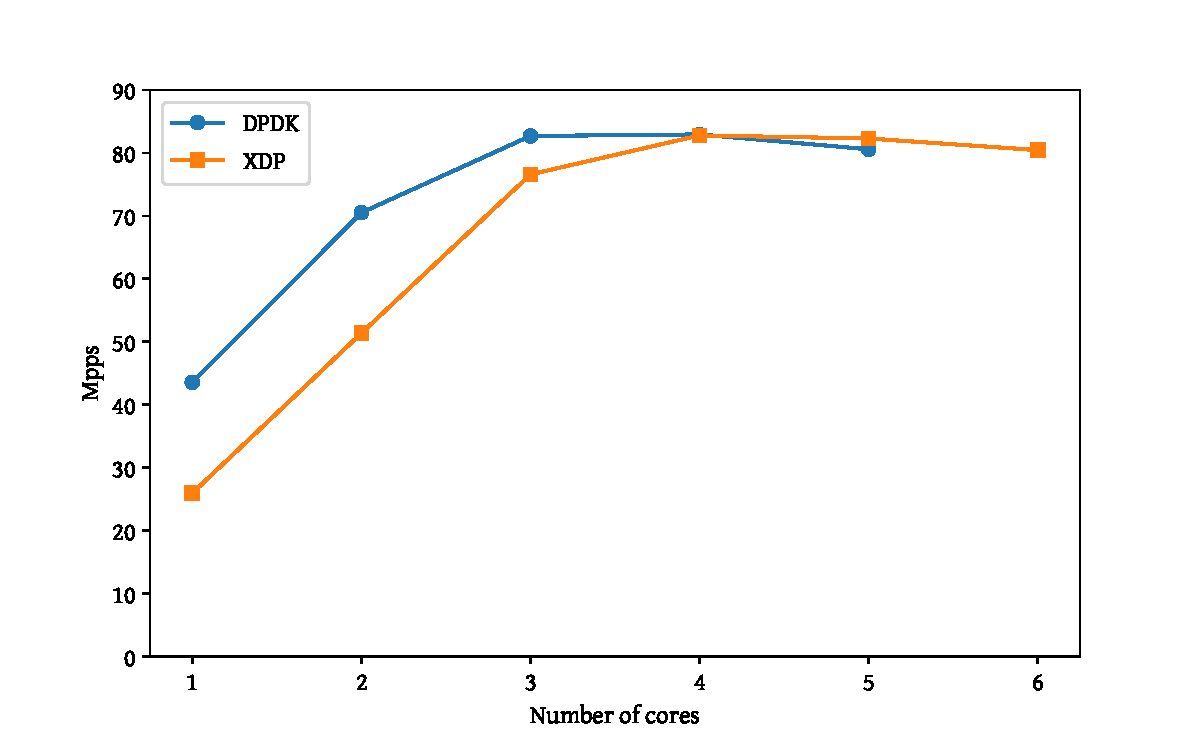
\includegraphics[width=\linewidth]{figures/drop-test.pdf}
\caption{\label{fig:drop-test} Packet drop performance. DPDK uses one core for
  control tasks, which is why it only goes to 5. The slight downward trend at
  above 4 cores is because the performance of our packet generator decreases
  when it has to generate more streams.}
\end{figure}


The hardware performance counters indicate that the global performance
bottleneck is the PCI bus capacity. The reason why DPDK achieves a higher
maximum performance before hitting the limit is that its busy-polling operating
mode allows it to make better use of the available capacity on the bus, while
the NAPI mechanism that the Linux kernel (and hence XDP) uses, intermittently
waits for interrupts, which leads to idle periods on the PCI bus.

The figure also shows the performance of the Linux networking stack in two
configurations: One where we use the ``raw'' mode of the \emph{iptables}
firewall module to drop packets, which ensures the earliest possible drop in the
network stack processing; and another where we enable the connection tracking
(\emph{conntrack}) module, which is enabled by default on most Linux
distributions, but which carries a high overhead. These two modes illustrate the
performance span of the Linux networking stack, from 1.8 Mpps of single-core
performance with conntrack, up to 4.8 Mpps in raw mode. It also shows that in
the absence of hardware bottlenecks, Linux performance scales linearly with the
number of cores. And finally, it shows that XDP offers a five-fold improvement
over the fastest processing mode of the regular networking stack, achieving 26
Mpps on a single core.


\subsection{CPU usage}
\label{sec:cpu-usage}

The CPU usage of the different tested systems, when configured to use a single
core and immediately drop packets, is shown in Figure~\ref{fig:drop-cpu}. The
test varies the offered packet load up to the maximum that each system can
handle on a single core. We then measure the percentage of CPU busy time using
the \texttt{mpstat} system utility.

Since DPDK by design dedicates a full core to packet processing, and uses busy
polling to process the packets, its CPU usage is always pegged at 100\%, which
is the green line at the top of the figure. In contrast, both XDP and Linux
smoothly scale CPU usage with the offered load, with a slightly larger relative
increase in CPU usage at a small offered load level.

\begin{figure}[t]
\centering
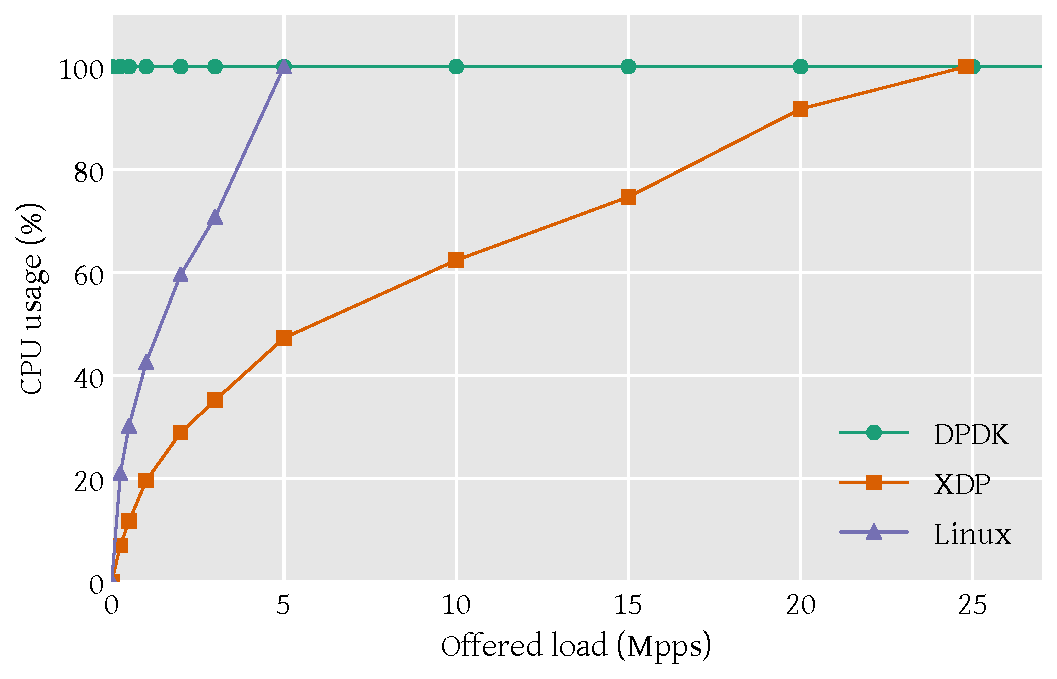
\includegraphics[width=\linewidth]{figures/drop-cpu.pdf}
\caption{\label{fig:drop-cpu} CPU usage in the drop scenario. Each line stops at
  the method's maximum processing capacity. The DPDK line continues at 100\% up
  to the maximum performance shown in Figure~\ref{fig:drop-test}.}
\end{figure}


\subsection{Packet Forwarding Performance}
\label{sec:pack-forw-perf}
Figure~\ref{fig:redirect-test} shows the packet forwarding performance. The
forwarding applications perform a simple Ethernet address rewrite, where the
source and destination address of the incoming packet are swapped before the
packet is forwarded. This is the minimum rewriting that is generally needed for
a real packet forwarding application, so the results represent an upper bound on
forwarding performance. Since XDP can forward packets out the same NIC as well
as out a different NIC (using two different program return codes), we include
both modes in the graph. The DPDK example program only supports forwarding
packets through a different interface, so we only include this operating mode in
the test. Finally, the Linux networking stack does not support this minimal
forwarding mode, but requires a full bridging or routing lookup to forward
packets; this lookup is expensive, and since the other applications don't
perform it, the results are not directly comparable. We instead include the
Linux routing performance in our real-world use case presented in
Section~\ref{sec:fwd-usecase}.

As Figure~\ref{fig:redirect-test} shows, we again see linear scaling the number
of cores up to a global performance bottleneck. The absolute performance is
somewhat lower than for the packet drop case, which shows the overhead of packet
forwarding. We also see that the XDP performance improves significantly when
packets are sent out on the same NIC that it came in on, especially as the
number of cores in use increases. This is primarily due to differences in memory
handling: packet buffers are allocated by the device driver and associated with
the receiving interface. And so, when the packet is forwarded out a different
interface, the memory buffer needs to be returned to the interface that it is
associated with, which has some overhead. Work is ongoing to reduce this
overhead.

\begin{figure}[t]
\centering
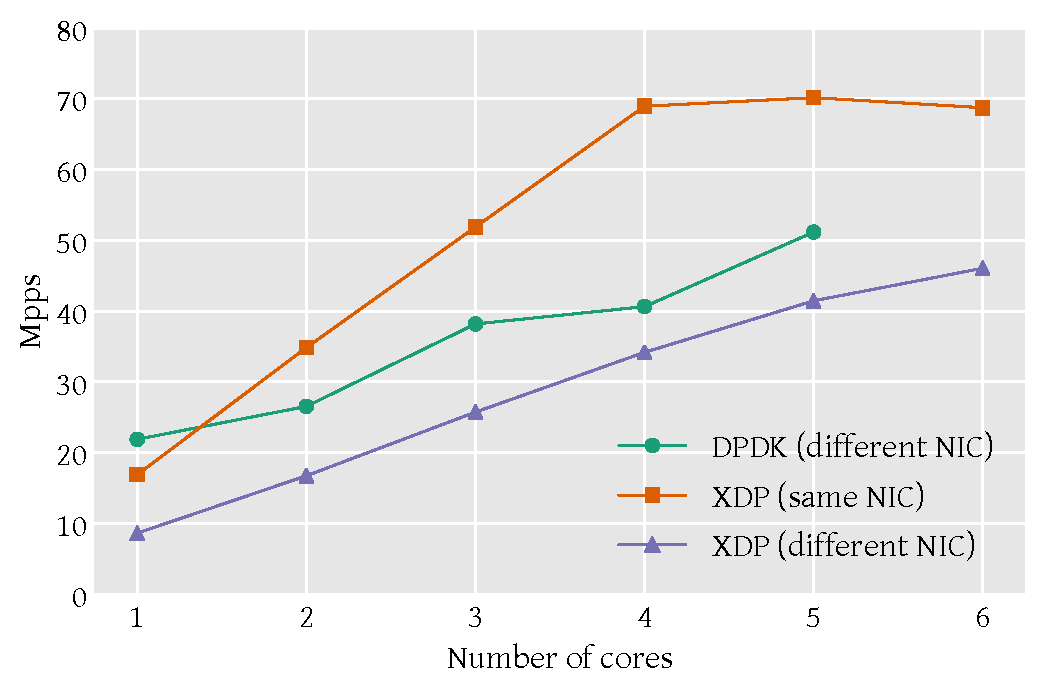
\includegraphics[width=\linewidth]{figures/redirect-test.pdf}
\caption{\label{fig:redirect-test} Packet forwarding performance. At 70 Mpps,
  the same-NIC performance is limited by the PCI bus (since RX and TX on the
  same device means only half the PCI slot bandwidth is available).}
\end{figure}

\subsection{Discussion}
\label{sec:perf-discussion}

As we have seen in the previous sections, XDP achieve significantly higher
performance than the regular Linux networking stack. Even so, for most use cases
XDP doesn't quite match the performance of DPDK. We believe this is primarily
because DPDK has incorporated more performance optimisations at the lowest level
of the code. To illustrate this, consider the packet drop example: XDP achieves
26\,Mpps, which corresponds to 38.4 nanoseconds per packet, while DPDK achieves
43.5\,Mpps, or 22.9 nanoseconds per packet. The difference of 15.5 nanoseconds
corresponds to 56 clock cycles on the 3.6\,Ghz processor in our test machine;
thus, it is clear that every micro-optimisation counts.

Specifically, we identify three areas where the performance of XDP can be
improved: (1) It is possible to eliminate some operations in XDP at the
architectural level, such as DMA map and unmap operations. (2) It is possible to
improve batching of operations, such as packet buffer returns across network
interfaces, and increasing the use of busy polling under heavy load. And (3),
there are some optimisations in the device driver code, such as inlining
function calls, that could be applied specifically to the mlx5 driver. Indeed
other drivers, such as the \emph{i40e} driver for 40\,Gbps Intel cards, show a
smaller performance delta between XDP and DPDK.

Given the above points, we believe it is quite feasible for XDP to close the
performance gap to DPDK completely. In addition, given the fact that this gap is
no longer a matter of orders of magnitude (as is the case between DPDK and the
regular Linux network stack), we believe that given its benefits in terms of
flexibility and integration with the rest of the system, XDP is already a
compelling choice for many use cases. We illustrate some examples of this in the
next section.

\section{Real-world use cases}
\label{sec:usecases}
To show how the various aspects of XDP can used to implement useful real-world
applications, this section gives three examples of such applications. These use
cases have all seen real-world deployment in one form or another, although we
use simplified versions in our evaluation so as to be able to make the code
available.

The first use case shows how XDP's kernel helpers can be used to accelerate
common use cases, using the example of a software router. In the second use
case, we show how an inline Denial of Service (DoS) mitigation application can
be used to protect against attacks directly at the application server. And
finally, the third use case shows how the XDP forwarding mode that sends packets
out the same interface as they arrived on can be used to implement a layer-3
load balancer.

\subsection{The Software Router Use Case}
\label{sec:fwd-usecase}
The Linux kernel contains a full-featured routing table, which includes support
for policy routing, source-specific routing, multipath load balancing, and more.
For the control plane, routing daemons such as Bird or FRR implement a variety
of routing control plane protocols. Because of this rich ecosystem built around
routing on Linux, improving performance of the kernel data plane is desirable;
especially since re-implementing the routing stack in another packet processing
framework carries a high cost.

XDP is a natural fit for this task, especially as it includes a helper function
which makes it possible to perform full routing table lookups directly from XDP.
The result of the lookup is an egress interface and a next-hop MAC address,
which makes it possible for the XDP program to immediately forward the packet if
the lookup succeeds. If no next-hop MAC is known (because neighbour lookup
hasn't been performed yet), the XDP program can instead pass the packet to the
networking stack, which will perform the neighbour lookup, allowing subsequent
packets to be forwarded by the XDP fast path.

To show the performance of this use case, we use the XDP routing example that is
included in the Linux kernel source~\cite{fwd-example} and compare its
performance to the regular Linux networking stack routing. We perform two tests:
one with a single route installed in the routing table and all packets set to
the same destination address. And another where we use a full dump of the global
BGP routing table from \emph{\url{routeviews.org}}, which we import into the
kernel routing table with all next-hop addresses set to the same value. The
routing table dump contains 752,138 distinct routes, and for our tests we
generate 4000 random destination IP addresses to make sure the full lookup table
is exercised.

The performance of this use case is seen in Figure~\ref{fig:router-fwd}. Using
XDP for the forwarding plane improves performance with a factor of 2.5 for a
full table lookup, and a factor 3 for the smaller routing table example. This
makes it feasible to run a software router with a full BGP table at full line
rate on a 10\,Gbps link using only two cores (using a conservative estimate of
an average packet size of 200\,bytes).

\begin{figure}[t]
\centering
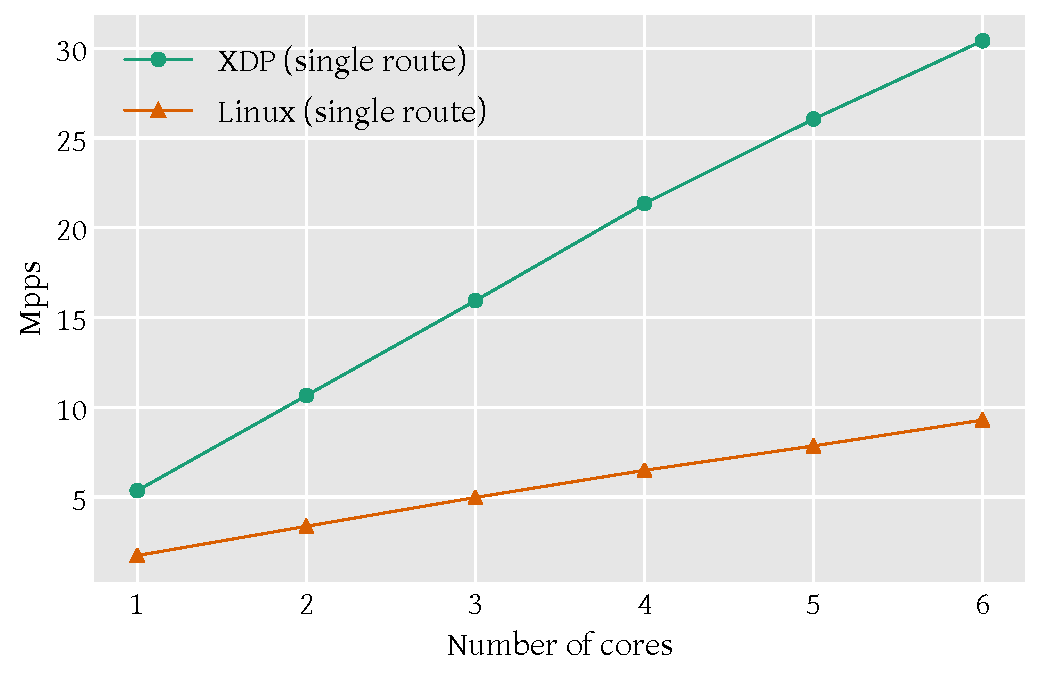
\includegraphics[width=\linewidth]{figures/router-fwd.pdf}
\caption{\label{fig:router-fwd} Software routing performance. Since the
  performance scales linearly with the number of cores, only the results for a
  single core are shown.}
\end{figure}

% See: (calc in benchmarks/bench04_fwd.org). The full-tables vs. single overhead
%  is signficantly larger than the expected overhead (according to Vincent
%  Bernat's measurements)
%  https://vincent.bernat.im/en/blog/2017-performance-progression-ipv4-route-lookup-linux

\subsection{Inline DoS Mitigation}
\label{sec:dos-usecase}
DoS attacks continue to plague the internet, typically in the form of
distributed attacks (DDoS attacks) from compromised devices attached to the
internet. With XDP, it is possible to deploy packet filtering to mitigate such
attacks directly at the application servers, without needing to change the
applications. In the case of a virtual machine deployment, the filter can even
be installed on the hypervisor, and thus protect all virtual machines running on
the host.

To show how this could work, we perform a test modelled on the DDoS mitigation
architecture used by Cloudflare, which uses XDP as the filtering
mechanism~\cite{cloudflare-ddos}. Their Gatebot architecture works by sampling
traffic at servers located in distributed Points of Presence (PoPs), collecting
it centrally for analysis, and formulating mitigation rules based on the
analysis. The mitigation rules take the form of a series of simple checks on the
packet payload, which are compiled directly into eBPF code which is distributed
to the edge servers in the PoPs and executed as an XDP program that will drop
packets matching the rules, while also updating match counters implemented as
BPF maps.

To test the performance of such a solution, we use an XDP program that parses
the packet headers and performs a small number of tests\footnote{A total of four
  tests are performed after the header parsing. For details, see the online
  appendix.} to identify attack traffic and drop it, and uses the CPU redirect
feature to pass all other packets on to the network stack for processing on a
different CPU core. To simulate a baseline application load we use the Netperf
benchmarking tool~\cite{netperf}, which contains a TCP-based round-trip
benchmark, which opens a TCP connection and sends a small payload which is
echoed back from the server, repeating as soon as a reply is received. The
output is the number of transactions per second, which is a good proxy for an
interactive TCP session, such as small remote procedure calls.

We run our experiment on a single core using a single hardware RX-queue.  This
creates the worst possible DoS situation, where good and bad traffic must
compete for the same hardware resources. We apply a baseline load of 35.000 TCP
transactions per second. We then offer an increasing load of small UDP packets
matching our packet filter, which simulates the DoS attack, and measure the
number of TCP transactions achieved as the attack traffic volume increases. We
repeat each experiment four times and report the mean value.

\begin{figure}[t]
\centering
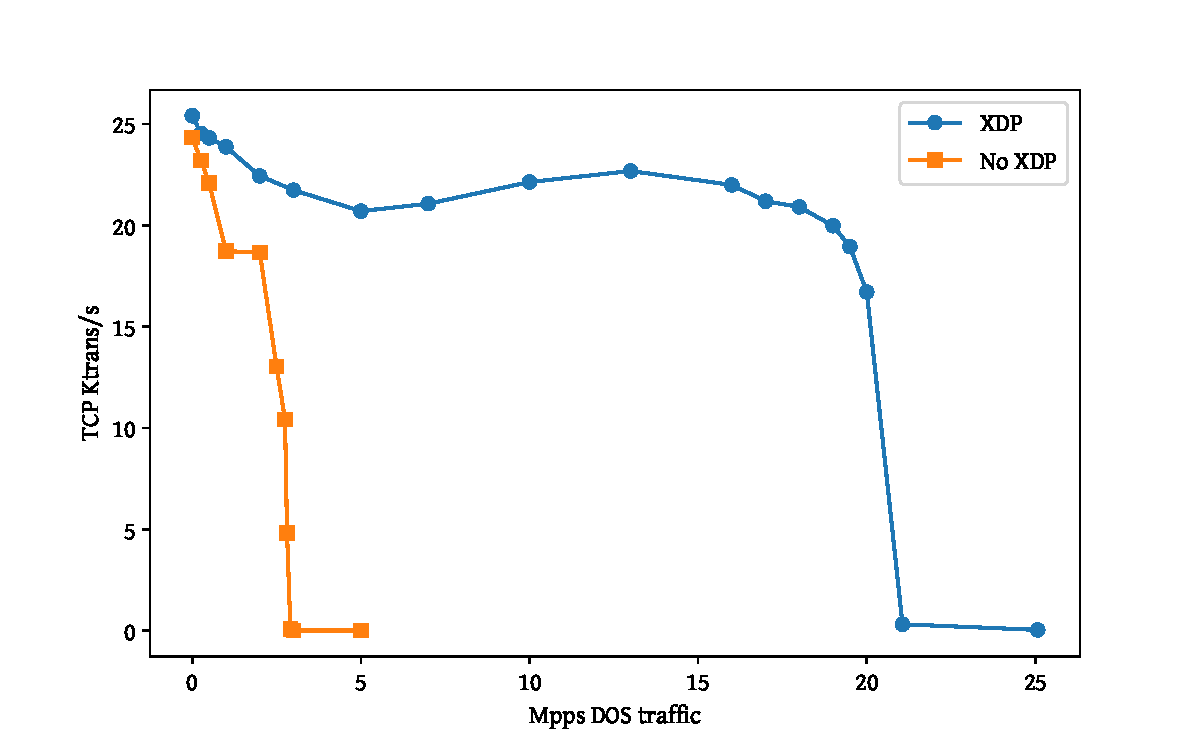
\includegraphics[width=\linewidth]{figures/ddos-test.pdf}
\caption{\label{fig:ddos-results} DDoS performance. Number of TCP transactions
  per second as the level of attack traffic directed at the server increases.}
\end{figure}

The results of this is shown in Figure~\ref{fig:ddos-results}. Without the XDP
filter, performance drops significantly, being halved at 3\,Mpps and effectively
zero at just below 3.5\,Mpps. However, with the XDP filter in place, the TCP
transaction performance is kept high, gradually increasing towards 25.000
transactions per second at 20\,Mpps, after which it drops rapidly. This shows
that effective DDoS filtering is quite feasible to perform in XDP, and
comfortably handles packet rates above 10\,Gbps of DoS traffic (with minimum
packet sizes) on a single CPU core. Deploying DDoS mitigation this way leads to
increased flexibility, since neither application changes, nor additional
hardware is needed.

\subsection{Load Balancer}
\label{sec:load-balancer}
For the load balancer use case, we use the XDP component of the Katran load
balancer~\cite{katran} recently released as open source by Facebook. This works
by announcing a virtual IP address to the world, which is then routed to the
load balancer. At the load balancer, the XDP program hashes the layer-4 packet
header using a stable hashing algorithm, which becomes a destination application
server. The packet is then encapsulated in a new IP header and sent to the
application server, which is responsible for decapsulating it, processing the
request, and replying directly to the originator of the request. This means that
the XDP program can perform the packet encapsulation, and immediately return the
packet out the same interface.

To test this use case, we configure the Katran XDP program with a fixed number
of destination hosts\footnote{We configure one virtual IP per CPU core, with 100
  destination application servers per virtual IP.}, and run it on our test
machine. Once the packets are returned to the network they are simply dropped;
we are only interested in the performance of the load balancer component itself.
This performance is shown in Table~\ref{tbl:load-balancer}, which, as in the
other examples, shows linear scaling with the number of CPUs, and the ability to
saturate a 10\,Gbps link using three CPU cores.

\begin{table}[htbp]
\caption{\label{tbl:load-balancer}Load balancer performance.}
\centering
\begin{tabular}{lcccccc}
  \toprule
  CPU Cores & 1   &  2  &  3  &  4  &  5  &  6  \\
  Mpps & 5.2 & 10.1 & 14.6 & 19.5 & 23.4 & 29.3 \\
\bottomrule
\end{tabular}
\end{table}




\section{Limitations and future work}
\label{sec:limitations}
As we have shown above, XDP has excellent performance, and is already useful in
a variety of real-world use cases. However, XDP is also relatively new
technology that is being incrementally added to a general purpose operating
system kernel. As such, it is constantly evolving, and still has some rough
edges. In this section we present some of the known limitations, and future
directions for XDP's development. These include: User experience and debugging;
driver support; improvements to NAPI; and better handling of rate transitions.
Each of the following subsections discuss each of these issues in turn.

\textbf{FIXME: This needs to strike the right balance between ``look, we are
  improving things'' and ``there are lots of issues''. I fear it leans a bit too
far towards the latter as is, so maybe some text needs to be cut.}

\subsection{User Experience and Debugging}
\label{sec:user-exper-debugg}
Since an XDP program runs in the kernel, the debugging tools available to a
regular userspace program are not generally applicable. The tendency for some
operations to fail silently and just drop packets doesn't help this situation.
In addition, the subset of C that is generally used to write BPF programs can be
limiting, for instance due to the need to unroll all loops. Finally, the
verifier will sometimes reject valid programs because it cannot prove validity,
and its error messages are not always helpful. Together, these issues combine to
make writing a useful XDP application harder than it needs to be, especially for
someone not familiar with the Linux ecosystem.

\textbf{FIXME: The issue is not so much that no debugging tools exist, but
  rather than it is a very different ecosystem.}

Work is ongoing to improve this situation, and indeed it already has improved
some. The XDP subsystem includes a number of tracepoints, that can be accessed
by the debugging tools used for the rest of the kernel to give information about
failures of XDP actions, usage of helper functions, etc. The tools to support
this continue to improve, as does the documentation. In addition, the verifier
continuously improving to recognise more correct programs that were previously
rejected as invalid. Support for function calls in eBPF has recently been added,
and the addition of support for bounded loops is planned. However, we recognise
that this is still an area in need of improvement.

\subsection{Driver Support}
\label{sec:driver-support}
Each device driver needs to add support for running XDP programs, by supporting
an API exposed by the core networking stack. Support is continuously being added
to more and more drivers.\footnote{At the time of writing Linux 4.17 has XDP
  support in 12 different drivers, including the most popular high-speed network
  adapters. An updated list of supported drivers is included in
  \url{http://cilium.readthedocs.io/en/latest/bpf}.} However, not having
universal support is limiting and can be confusing for users. One particular
issue with this is that it is possible for drivers to support only subsets of
the XDP functionality. This is because drivers need to implement support for
each of the possible return code. This is further complicated by the fact that
support for redirection has separate implementations in the receive path and the
transmit path, so it is possible for a driver to support redirecting packets to
other interfaces, but not being the target of a redirection from elsewhere.

Ultimately, we believe that these issues will be resolved by having full support
for XDP in all device drivers. However, for obvious reasons this takes time, and
holding back the development of the system until all drivers have caught up is
not feasible. As the XDP system has evolved, the need to keep the API support
required in drivers to a minimum has become increasingly clear, and some steps
have been taken in this direction. For instance, support for new targets can be
added to the redirection action without any changes needed from the drivers.

\textbf{FIXME: Mention closing the performance gap with DPDK.}

\subsection{Improvements to NAPI}
\label{sec:improvements-napi}
As we saw in Section~\ref{sec:perf-eval}, DPDK still achieves markedly better
raw packet processing performance than XDP. The main reason for this is that the
NAPI mechanism that Linux uses to selectively switch between interrupt-based
packet processing and polling is insufficient to mitigate the large number of
interrupts that happen at high packet rates. In some cases it would be
beneficial to switch to a full busy polling mode, if one is willing to dedicate
a full CPU core to packet processing.

There have been some efforts to selective switch a network adapter to busy
polling mode, which has shown promising results~\cite{dumazet17:_busyp}. We
believe continuing this work, and integrating it with XDP, will make it possible
to reach raw packet processing performance equal to that of DPDK.

\subsection{QoS and Rate Transitions}
\label{sec:handl-rate-trans}
Currently, XDP does not implement any mechanism for supporting different Quality
of Service (QoS). Specifically, an XDP program receives no backpressure when
attempting to forward packets to a destination that has exhausted its capacity.
This limitation can be exasperated when joining networks with different speeds
or other mismatched network characteristics.

We are exploring various solutions to this issue, however no consensus on the
best approach has been reached in the community at this time.


\section{Conclusions}
\label{sec:conclusion}
We have presented XDP, a system for safely integrating high-speed programmable
packet processing directly in the Linux kernel. This represents an alternative
solution to all-or-nothing kernel bypass solutions, which makes it easier to
integrate the packet processing with normal applications.

Our evaluation has shown that XDP achieves raw packet processing performance of
up to 25 million packets per second on a single CPU core. We have also
demonstrated three examples of real-world use cases that can be implemented with
XDP: Inline DDOS mitigation, layer-3 forwarding, and layer-4 load balancing.

XDP continues to be actively developed by the Linux community, and we believe
that it offers a compelling alternative to other high-speed packet processing
frameworks, especially where integrating with existing systems and applications
is important.

\bibliographystyle{ACM-Reference-Format}
\bibliography{xdp}

\end{document}
